\chapter{Methodology}

The usage of alert data with Machine Learning algorithms suffers from two issues; significant preprocessing must be performed to make the data have contextual meaning and methods to analyze the similarity of alerts are not well defined. For example, predicting a specific port which will be attacked only provides a small piece of significant data. However, a more significant feature to generate would be what type of service is typically run on a family of ports so that similar ports are grouped together. Additionally, when analyzing cyber alerts identifying the fidelity of data is not straight forward. In tasks such as event prediction results may be quantified by cross entropy loss on a per feature basis. But when generating new alerts there are complex interactions between various features which must be accounted for by the model. Simply generating \emph{a} realistic signature and port category is much less important than generating a realistic \emph{combination} of port signature and category. 

To address these challenges this section will cover the unique preprocessing applied to NIDS data collected from Suricata. Specifically, the features of alert signature, destination port, timestamp, and source IP will be considered. Additionally, intuitive metrics for analyzing alert fidelity are introduced as an inclusive system to address how realisitc generated alerts are compared to their source alerts from the ground truth dataset. 

\section{Cyber Alert Data Preprocessing}


The data used for these experiments comes from the National Collegiate Penetration Testing Competition from 2017 and 2018 (\texttt{https://nationalcptc.org/}). In 2017, teams were tasked with penetrating and exploiting network vulnerabilities in a virtualized network managing election systems. In 2018 teams were required to attack a multifaceted system handling autonomous cars which included host based systems, servers, and even mobile assets such as cell phones running an app. Each team had a total of 8 hours to scan, infiltrate, and exfiltrate information from the network. Both datasets provide a unique opportunity for Machine Learning experimentation as they are completely comprised of malicious actions as teams attempt to penetrate the target network. Though this data is unique to the competition it is worth noting that the preprocessing described herein is applicable to any dataset consisting of NIDS alerts.  

The first preprocessing step applied to the data was to separate alerts on a per-destination/target IP basis. This allowed individual models to be trained for each system on the network, typifying the type of traffic seen at that node. Additionally, data from all of the teams could be compounded, allowing for the number of potential attacks taken on a single target to be more fully expressed during training. Segmentation on a per-target basis has several intuitive benefits: First, it allows for different vulnerabilities to be highlighted on each machine given commonly occurring alert features at that target. Secondly, it helps to remove noisy alert influence from critical nodes in the network. For example, internet facing IPs may contain a significant amount of scanning activity, drowning out exfiltration related alert features at nodes further embedded in the network. Finally, the information extracted from alerts on a per target basis is actionable, as network administrators can use commonly targeted vulnerabilities to tune network settings for future defenses. 

% TODO: Numbers are for CPTC17 only -update with table

Next, the dimensionality of the destination port feature was reduced based off common service categories run across a collection of ports provided by the Internet Assigned Numbers Authority \cite{iana}. This reduction drops the number of unique values from 1516 destination ports to 69 destination port categories. Additionally, the dimensionality reduction step can easily be expanded or customized on a per network basis given a corporation's configuration of services. 

% TODO: Duplicate alerts are removed for 17, but not for 18. -retest


Finally, a set of simple statistical criterion are used to segment timestamps into bins. Traditional modeling of cyber attacks use killchain stages to segment actions into a series of contiguous stages with dependencies on previous stages. The beginning of an attack may consist of Reconnaissance based actions, yielding information about which IP to target in later attack stages. Similarly, the CPTC dataset may be segmented to try and capture unique behaviors into different bins of time. 

If applied to real world NIDS data another potential preprocessing step would be to segment source IPs based off of subnet. However, given that CPTC occurs in a virtualized network for a collegiate competition this preprocessing step is ignored. 

Following the methodology shown by \cite{us} bins are generated by smoothing the histogram timestamps and taking the first derivative to identify local minima and maxima. Then stages are cut if they contain at least $10\%$ of the total data and consecutive events at the candidate point contain less than $0.5\%$ of the total data. The goal of this ruleset is to capture significantly different types of traffic that does not split bursts of data into multiple stages. This process is shown visually in Fig. \ref{fig:cut_process}.



\begin{figure}[!htbp]
	\centering%
	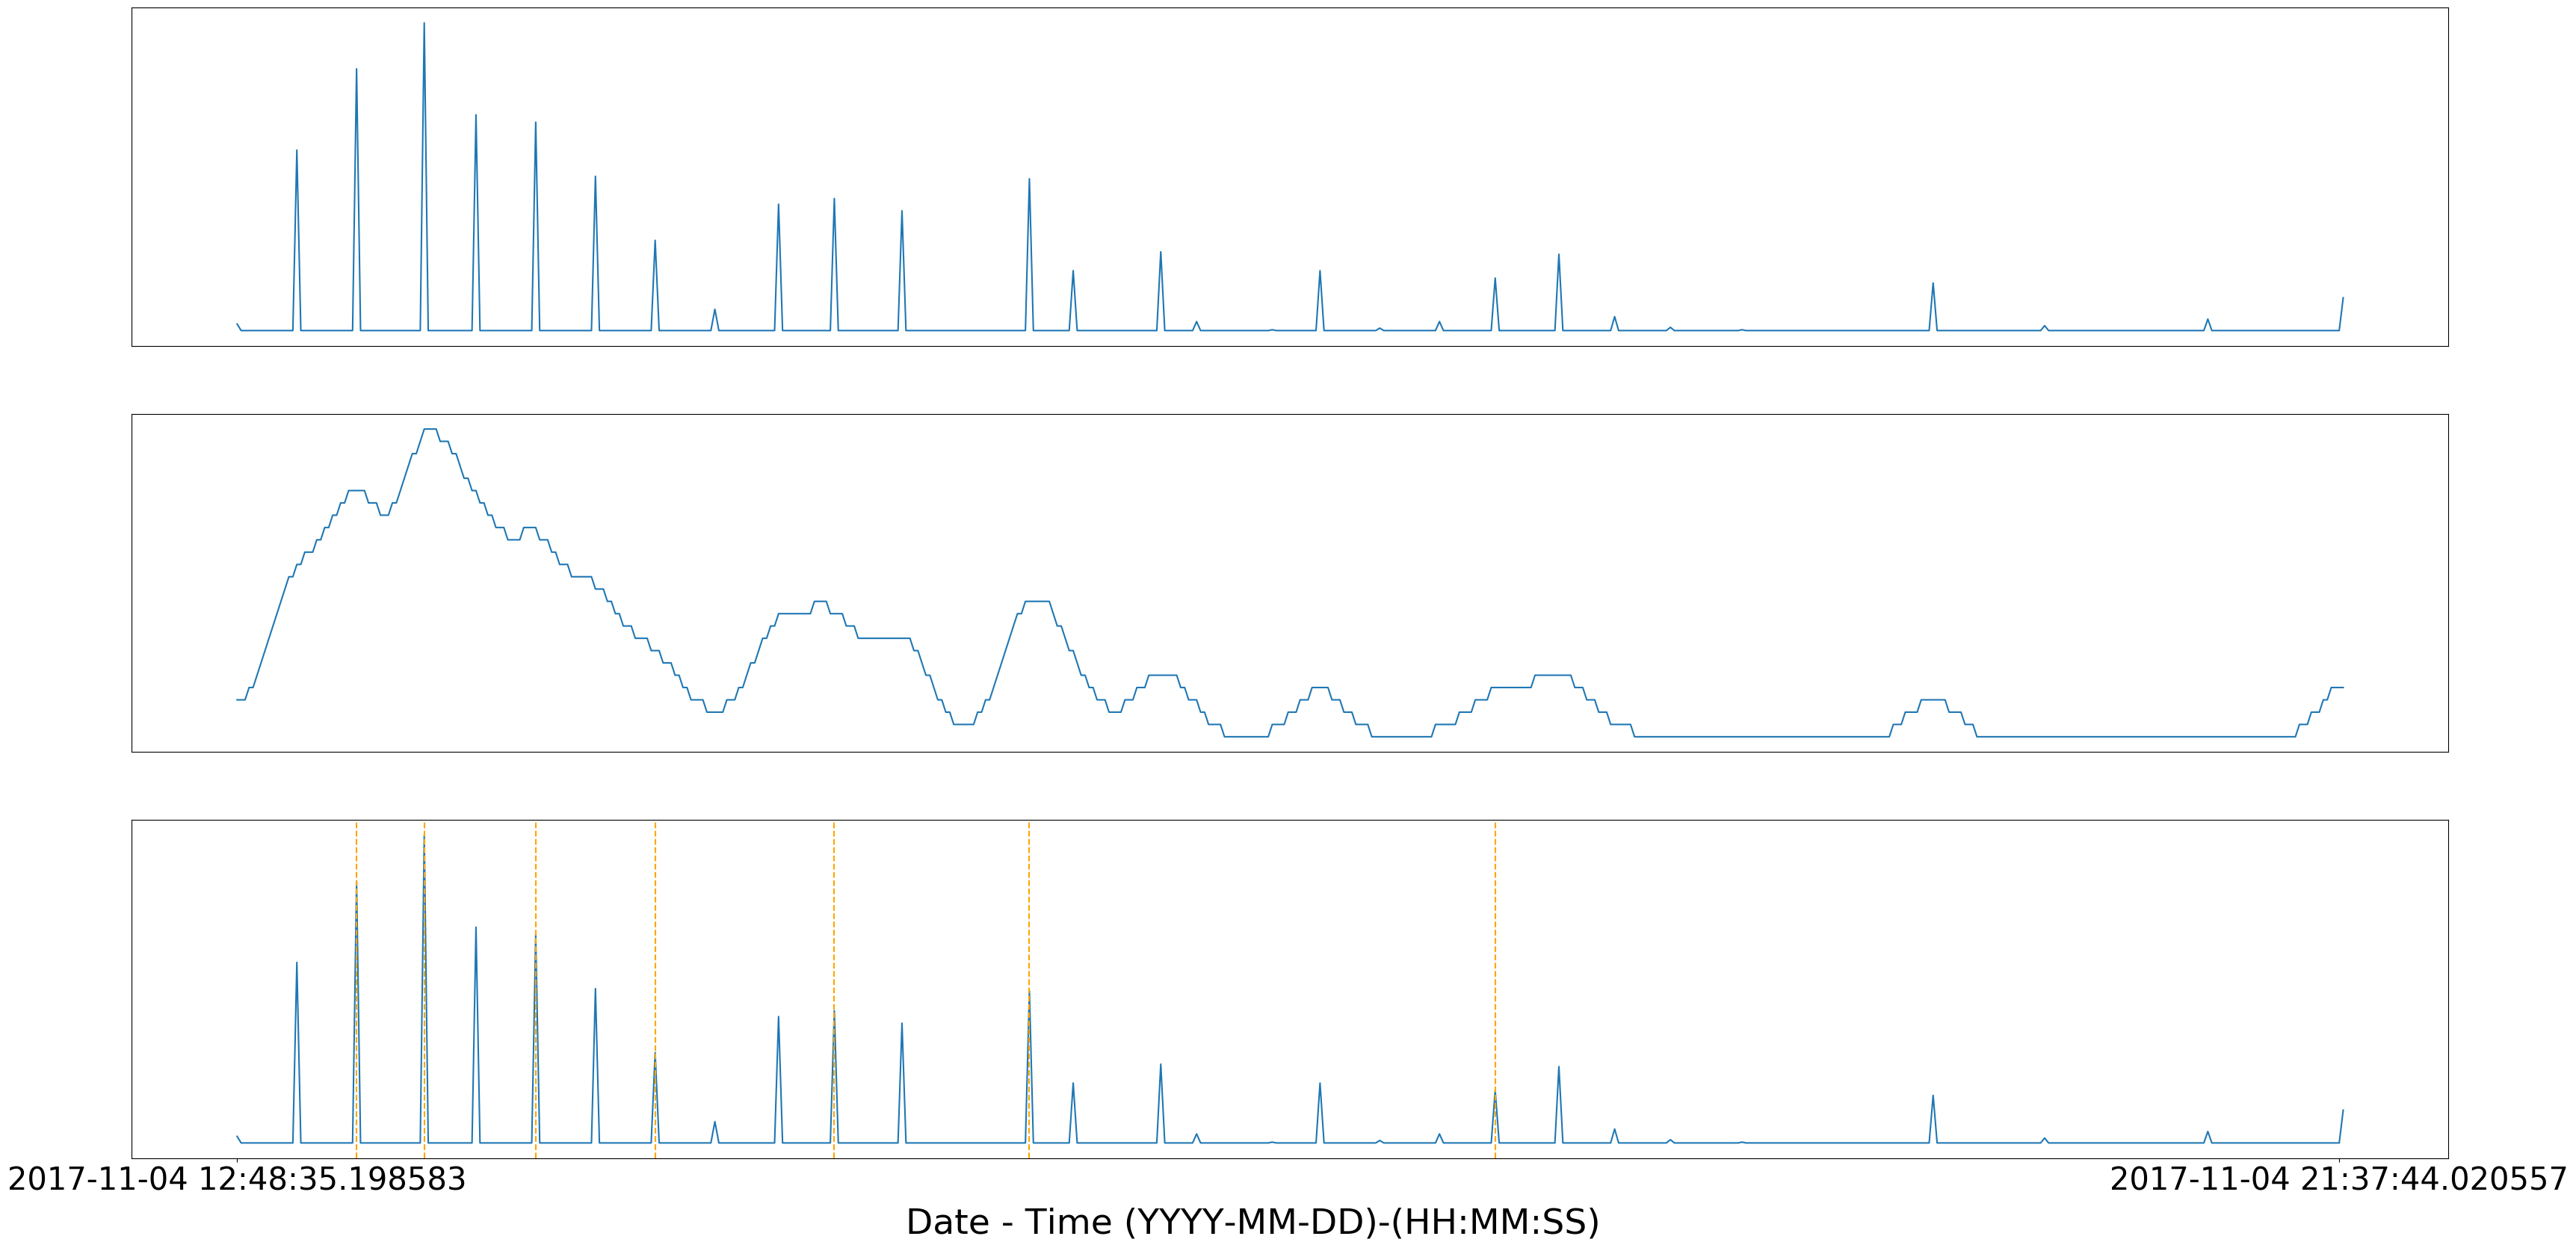
\includegraphics[width=\textwidth]{10_0_0_22_cuts}
	\caption{
		(Top) Raw plot of timestamp influx.
		(Middle) Gaussian smoothed timestamps.
		(Bottom) Original timestamp influx with lines indicating stage separation. 
	}
	\label{fig:cut_process}
\end{figure}

\section{Methods of Analyzing Alert Data}

Analyzing the degree of realism for artificially generated alert data is non-trivial. While other fields such as Computer Vision have created well defined metrics such as Inception Score \cite{Salimans2016} or allow for direct human analysis of image quality, no analogue exists for NIDS alerts. Several works have proposed the use of graph based metrics such as comparing nodes and their connectivity for both generated and real network traffic \cite{Siska2010, Iannucci}, or looking at low level parameters such as distributions of packets \cite{Sommers2004, Botta2012}. However, despite these works there is no widely accepted methodology.

It is important to consider the desirable attributes of a \emph{good} metric. A good metric must provide an intuitive, scalable way to summarize what would otherwise be an intractable amount of data to comprehend. Other desirable properties include ways to directly visualize the results of the metric so that trends may be identified visually, able to capture high level dependencies, and tolerance to samples with the value $0$. 

To this end, we propose the usage of several metrics for analyzing NIDS alert data. First, histogram intersection; this metric compares the similarity of two histograms within the same domain by computing the amount of overlap between them. Histogram intersection meets several of the above criterion, as it is naturally bounded between 0 and 1, easily visualized by directly plotting the histograms being compared, and can be extended to accommodate m-many tuples of features. The m-many tuples can be thought of as a joint histogram, where $m$ is the number of unique features considered in the joint. This can be done automatically by iterating over all $M$ choose $m$ \emph{combinations}, where $M$ is the total unique features in the dataset. Mathematically histogram intersection is defined in (\ref{eq:intersection}), where \emph{gt} represents the ground truth data histogram and \emph{gen} represents the generated data histogram, each of which has $N$ samples.

\begin{equation}
\label{eq:intersection}
	G = {{\sum_{i=0}^{N} min(gt_i, gen\_i)} \over {max(\sum_{i=0}^{N} gt_i, \sum_{i=0}^{N} gen_i)}}
\end{equation}

Another powerful trait of histogram intersection is that it can be used to reveal dependencies between features within a single alert. This is accomplished by looking at the difference in histogram intersection scores between $n\pm1$ tuples and observing the intersection drop. An intuitive example of this can be thought of as follows; If the intersection for feature $A$ is 0.9 and the intersection for a 2-tuple histogram consisting of features $A$ and $B$ is $0.875$ then it is expected that a dependency exists between $A$ and $B$. It is important to note that this dependency is not inherently bidirectional, as $A$ and $B$ may have varying intersections to begin with. Fig. \ref{fig:metric_graph} illustrates a graph based schema to identify these dependencies visually. 

\begin{figure}[!htbp]
	\centering%
	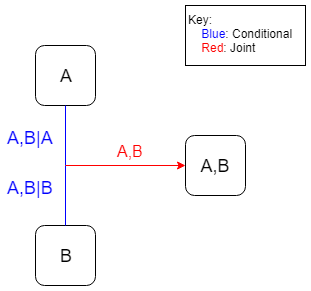
\includegraphics[width=70mm]{metric_graph}
	\caption{
		Note that along the edges heading from Nodes A and B are the conditional entropy term may be visualized. The point where the two segments join and travel to the node labeled A,B represents the joint entropy term.
	}
	\label{fig:metric_graph}
\end{figure}

In order to confirm these dependencies we introduce our second metric; conditional entropy. The conditional entropy of each unique \emph{permutation} may be calculated for each m-tuple of features. Continuing with the previous example this means the conditional entropy of both $A|B$ and $B|A$ are computed. In order to compute a single value that represents the average conditional entropy for all input condition values, the entropy term is computed using (\ref{eq:wce}). This calculation weights the entropy of each possible input combination based off the probability that input $i$ occurs as ${{|w_i|} \over {|w|}}$. ${p_{i|j}}$ represents the probability of the output feature value at index $j$ occurring given the input feature values at index $i$ and must be computed for possible output values $Z$.

\begin{equation}
\label{eq:wce}
\widehat{H}_{Y|X_0, X_1, ..., X_m} = \sum_{i=0}^{N} \bigg({{|w_i|} \over {|w|}} * {\sum_{j=0}^{Z}\Big({p_{i|j} * \log ({1 \over{p_{i|j}}})}\Big)}\bigg)
\end{equation}

In order to further strengthen the argument that there are dependencies between features it is important to consider the overall randomness of the m-tuple joint distribution. To do this (\ref{eq:je}) may be used to compute the joint entropy of the distribution. Using the aforementioned example with features $A$ and $B$, the joint of these variables is denoted $A,B$.

\begin{equation}
\label{eq:je}
{H}_{X_m} = -\sum_{x_m} p(x_0, x_1,...,x_m)  * \log \big({{p(x_0,x_1,...,x_m)}}\big)
\end{equation}

Given that natural logarithms are used for the calculation in (\ref{eq:wce}) and (\ref{eq:je}), the resulting value is given in the natural unit of information (nats), a log base e equivalent to bits. Given that the distribution of m-tuple feature histograms is a discrete distribution with finite support the upper bound of entropy is given by the uniform distribution $mathbb{U}$. Note that the cardinality of $mathbb{U}$ varies to match the number of unique values in the conditional or joint probability being normalized. Using this quantity (\ref{eq:wce}) can be normalized as shown in (\ref{eq:norm_wce}) and (\ref{eq:norm_je}). This has the benefit of naturally bounding the entropies between 0 and 1, similar to the intersection score defined in (\ref{eq:intersection}).


\begin{equation}
\label{eq:norm_wce}
\overline{H}_{Y|X_0, X_1, ..., X_m} = {{\widehat{H}_{Y|X_0, X_1, ..., X_m}} \over{ H(\mathbb{U})}}
\end{equation}


\begin{equation}
\label{eq:norm_je}
\overline{H}_{X_m} = {{{H}_{X_m}} \over{ H(\mathbb{U})}}
\end{equation}

If the drop in intersections is indeed correlated to feature dependency, then the conditional entropy should be directly proportional to this drop. Additionally, the benefit of capturing feature dependencies is apparent by comparing to the joint entropy without any conditioning information. Note that in Fig. \ref{I haven't made this yet} the edges corresponding to conditional and joint entropies are labeled using the notation given in the examples above.

One drawback of using the intersection of histograms is that the metric does not perform well when the ground truth distribution evaluated is highly deterministic. The data generating model can learn to output that value in a purely deterministic manner and receive an intersection score equivalent to the probability of that given value occurring in the ground truth set. In order to avoid this issue a metric which penalizes failure to encompass the entire domain of output values. 

Kullback Leibler (KL) divergence was considered as a candidate, however it does not have the property of zero tolerance and is asymmetric. However, the Jensen Shannon (JS) divergence is both zero tolerant and symmetric. This metric has the downside of having no upper bound and by extension is not as intuitive as the previously proposed metrics with firm bounds. This metric can be used as a drop in replacement for the histogram intersection and still be used in conjunction with the weighted conditional and joint entropies.

\subsection{An Aside: Using Conditional Probability Tables to Evaluate Generated Alerts}

In the aforementioned (\ref{eq:wce}) weighted conditional entropy is computed to provide a singular score representing conditional randomness in m-tuple histograms. An intermediary step in this computation involves the creation of conditional probability tables which show all possible input conditioning values and their impact on output value probability. It was found through experimentation that directly outputting these tables and applying highlighting to reveal sparsity and determinism is an effective means to evaluate specific feature value relationships. This method has the drawback of becoming intractable as the number of tables generated is equal to the number of unique feature permutations. A sample table is given in Section \ref{sec:rna} to illustrate this point. 
